\documentclass[conference]{IEEEtran}
\IEEEoverridecommandlockouts
% The preceding line is only needed to identify funding in the first footnote. If that is unneeded, please comment it out.
\usepackage{cite}
\usepackage{amsmath,amssymb,amsfonts}
\usepackage{algorithmic}
\usepackage{graphicx}
\usepackage[export]{adjustbox}
\usepackage{wrapfig}
\usepackage{graphicx}
\usepackage{hyperref}
\usepackage{todonotes}
\usepackage{subcaption}
\usepackage{nameref}
\usepackage{graphicx}
\usepackage{subcaption}
\usepackage{hyperref}
\usepackage{amsmath}
\usepackage{hyperref}
\usepackage{xcolor}
\usepackage{placeins}
\renewcommand*{\figureautorefname}{Fig.}
\def\BibTeX{{\rm B\kern-.05em{\sc i\kern-.025em b}\kern-.08em
    T\kern-.1667em\lower.7ex\hbox{E}\kern-.125emX}}
\begin{document}



\title{Towards Generalization of Bipedal Gait Cycle During Stair Climbing using Learning from Demonstration}
% \author{\IEEEauthorblockN{\textbf{Nathaniel Goldfarb}}
% \IEEEauthorblockA{\textit{Robotics Engineering} \\
% \textit{Worcester Polytechnic Institute}\\
% Worcester, MA, USA \\
% nagoldfarb@wpi.edu}
% \and
% \IEEEauthorblockN{\textbf{Charles Bales}}
% \IEEEauthorblockA{\textit{Robotics Engineering} \\
% \textit{Worcester Polytechnic Institute}\\
% Worcester, MA, USA  \\
% csbales@wpi.edu}
% \and
% \IEEEauthorblockN{\textbf{Gregory S. Fischer}}
% \IEEEauthorblockA{\textit{Robotics Engineering} \\
% \textit{Worcester Polytechnic Institute}\\
% Worcester, MA, USA  \\
% gfischer@wpi.edu}
% }


\author{Nathaniel Goldfarb$^{1}$, Charles Bales$^{1}$, and Gregory S. Fischer$^{1} $ % 
\thanks{Manuscript received \today}%
\thanks{This work does not have external financial support}%
\thanks{$^{1}$ Robotics Engineering Department at Worcester Polytechnic Institute, 85 Prescott St, Worcester, MA 01609 {\tt\small nagoldfarb@wpi.edu}}%

}

\maketitle


\begin{abstract}


Lower limb assistive exoskeletons for rehabilitation is a growing field of study. They allow people with spinal cord injuries and strokes to stand upright and walk. Exoskeleton controls research typically focuses on trajectory generation, motion control over the trajectories, and balance and stability. This work focuses on the generalization of people's joint trajectories climbing a single stair, for an exoskeleton to be developed for people of all leg lengths and be used on variable stair heights. The motion of subjects of different heights, ages, and genders climbing a single stair was collected using motion capture. By using Gaussian mixed regression and Gaussian mixed models, these trajectories were combined to build a model that generalizes individuals with different leg lengths, genders, ages and stair heights. The variability of the subject's leg length is accounted for by tracking a marker on the toe of the subject and using inverse kinematics to calculate the joint angles. The analysis in this paper shows that joint angles can be generalized to climb various stair heights. In addition, an open-source database of motion capture climbing data and an open-source framework for generating joint trajectories has been made available for public use.



% Rehabilitation exoskeletons are a growing field of study, and research shows they can provide benefits for people with spinal cord injuries and strokes. To be effective as a locomotive aid, lower-limb exoskeletons must accurately reproduce human gait over a range of terrain and obstacles commonly encountered during daily life. Exoskeletons' control is typically divided into two layers: trajectory generation and motion control over the trajectories. This work focuses on the former, the generation of the joint trajectories. In this paper, the motion of several subjects of different heights, ages, and genders climbing stairs was collected using motion capture. The variability of the subject's leg length is accounted for by tracking a marker on the toe of the subject then using inverse kinematics to calculate the joint angles. By using Gaussian mixed regression and Gaussian mixed models, these trajectories can be combined to learn a model that generalizes to individuals with different leg lengths and stair heights. This paper presents an open-source database of mocap climbing data, an open-source framework for generating joint trajectories for people with different leg lengths and stair heights, and verification of the framework using the provided data.




% Spinal cord injuries result in lower limb paralysis resulting in a reduced quality of life. Rehabilitation lower limb exoskeletons are a growing field of study, and research shows they provide relief for people with spinal cord injuries. These exoskeletons need to be able to replicate human motion to avoid putting extra stress on the joints. Exoskeletons control is divided into two fields of study: the dynamic control and trajectory generation. This work focuses on the latter, the generation of the joint trajectories.  The human motion of stair climbing was collected using a motion capture system. By exploiting learning by demonstration, this data can be used to learn and generalize. By using Gaussian mixed regression and Gaussian mixed models, these trajectories can be combined to learn a model. The model can then be used for people with different leg lengths. Additionally, this model can be used to climb upstairs from different heights. The generalization also allows for joint constraints and underactuated systems. This paper presents a model to generate joint trajectories that can be used for subjects of varying heights and can be dynamically changed on the fly to climb stairs of different heights.    
\end{abstract}
\begin{IEEEkeywords}
Learning from Demonstration, Exoskeletons, Trajectory Generation,  Gaussian Mixed Models
\end{IEEEkeywords}
%\section{Introduction}
Exoskeletons and biped robots share many similarities, but exoskeletons have additional constraints. They have to interface with a person who imposes the joint biological limits on the system. The exoskeleton joints should be co-linear with the person and avoid skin irritation. These constraints should be considered when designing a controller for a lower limb exoskeleton. The exoskeleton should comply with human movement to provide a more comfortable fit and make it easier to use.

Lower limb assistive exoskeletons need to be able to navigate different types of terrain found in everyday living. Systems such as, the Rewalk \cite{esquenazi2012rewalk}, the Esko \cite{mertz2012next}, and the Vanderbilt exoskeletons \cite{gasser2017design} have presented promising results; their systems enable people with spinal cord injuries (SCI) and other neurological conditions to stand and walk with assistance \cite{farris2013preliminary}. Both walking and stair climbing are activities of daily living (ADL). Stair climbing is considered a hazardous form of locomotion \cite{HicksLittle2011LowerEJ}  due to the potential for the foot to collide with the stair if the trajectory is incorrect. 

Two fields of interest in lower limb exoskeleton control are the controller's design and the trajectory planner \cite{huang2016optimisation}. These two fields are highly related; the controller produces the torques, while the trajectory generation generates the path for the leg to follow. This work focuses on the generation of the trajectory from the start to the goal, not taking into consideration balance and stability. This research assumes that the goal point is within the exoskeletons support polygon using zero moment point \cite{kajita2003biped}. Exoskeletons directly interface with a person's body and need to  follow the user’s natural joint movement; if this motion does not appropriately match, then there is an excess strain on the person’s joints. The lower level motion controller handles the variation of the mass of the person and the contact dynamics with the environment, while the trajectory generation follows natural motions.

The following paper proposes a learning from demonstration model that uses human motion data. As part of this study, motion capture trials were conducted to collect the necessary data of people of different masses, heights and genders. This data was segmented to extract the motion of climbing the first stair from the floor. The marker on the toe represents the footpath over the step motion while inverse kinematics calculates the joint angles. This structure allows the imitation model to handle various people and stairs of different heights.

The collected data was used to find the general trajectory to climb a stair. Using Gaussian Mixed Model (GMM), the trajectories were encoded into radial basis functions (RBF) placed throughout the data set. The forcing function is found using Gaussian Mixed Regression (GMR), which regresses over the RBFs. This forcing function is used to drive the Dynamic Movement Primitives (DMP) model. This procedure allows for manipulation for temporal, start, and goal manipulation.

\begin{figure} 
    \centering 
    \includegraphics[scale=0.2]{images/demo_figure.png} 
    \caption{Order of operations of the learning process. The data is collected, the demos are encoded, the model is retrieved, then the model is reproduced.} 
    \label{fig:demostation} 
\end{figure} 


This model shows that there is no need to retrain the trajectory for each person and different stair heights. To increase the data in the community, all data used is available online\footnote{\url{https://github.com/WPI-AIM/AIM\_GaitData}}. Increased public data will help the community develop and study human motion.
%\input{sections/background}

\bstctlcite{IEEEexample:BSTcontrol}

%\section{Introduction} 

Assistive exoskeletons are a growing field of study. Systems like the Rewalk \cite{esquenazi2012rewalk}, Esko \cite{mertz2012next}, and Vanderbilt exoskeletons \cite{gasser2017design} have presented promising results; their systems enable people with spinal cord injuries (SCI) and other neurological conditions to stand and walk with assistance \cite{farris2013preliminary}. The trajectory generation is essential so that joints follow natural motions. The lower level motion controller handles the variation of the mass of the person and the contact dynamics. Exoskeletons directly interface with a person's body. The joint movement control closely follows the user’s natural joint movement; if this motion does not appropriately match the user's joint motion, then there is an excess strain on the person’s joints.

The exoskeleton should move in an anatomically correct manner. Both walking and stair climbing are activities of daily living (ADL). Stair climbing is considered a hazardous form of locomotion \cite{HicksLittle2011LowerEJ}  due to the potential for the foot to collide with the stair if the trajectory is incorrect.  

Two fields of research in lower-limb exoskeleton control are the controller's design and the trajectory controller \cite{huang2016optimisation}. These two fields are highly related; the controller produces the torques, while the trajectory generation moves the joints and ensures that the placement of the foot is in a stable position. There is a significant amount of work on detailing how to teach a robotic system how to walk. Teaching a robot to follow a task is challenging; it involves balancing leg trajectory generation, single-leg support, and double-leg support.

Additionally, in \cite{taskjointmocap}, Hu \textit{et. al} focused on online generations of trajectories. They formulated the control problem as a Quadratic Programming (QP) problem, and the authors used both Cartesian and joint data as the imitation criteria. The formulation as a QP problem allows for inequality and equality constraints for the knee velocity. This formulation resolves the conflicts between the joint space and the Cartesian imitation data. This method is limited to level ground walking. This process did not address the problem of abstracting the trajectories for different stair heights; it only addresses level ground walking and fully actuated systems.

Able-bodied people have the innate ability to adapt and adjust to their environment. When they encounter stairs of different heights, they can ascend them without issue. For exoskeletons to climb stairs, they need to have the same ability to adapt to different stair heights. This paper presents a model to allow exoskeletons to adapt their motion to different stair heights. The motion capture system (mocap) records joint kinematics during stair ascent to build a library.

Stair climbing is a non-linear task that engages multiple muscle groups and requires balancing the torso. Ascending stairs requires one foot to remain on the ground while the other foot swings through a trajectory\cite{hicks2012temporal}. Several studies have examined how people climb upstairs. Motion capture is one tool that can be used for recording human kinematics and kinetics. In  \cite{chalodhorn2007learning}, Chalodhorn \textit{et. al} used a model-free approach to teach a robot to walk.
In  \cite{hu2014online}, Hu \textit{et. al} used quadratic programming to optimize the mapping of the markers to the robot. In both cases, the motion capture mapping was mapped from a human to a humanoid robot. Although exoskeletons and biped robots share many similarities, exoskeletons have additional constraints. They have to interface with a person who imposes the joint biological limits on the system. The exoskeleton joints have to be co-linear with the person and avoid skin irritation. These constraints should be considered when designing a controller for a lower limb exoskeleton. The exoskeleton has to comply with human movement.

The work conducted in \cite{andriacchi1980study} and \cite{hicks2011lower} focused on the kinematics and dynamics of stair climbing by using a combination of motion capture, force plates, and IMUs sensors. These studies have produced high-resolution joint angle data for level ground walking and stair climbing.

%\subsection{Learning from Demonstration}  

Learning from Demonstration (LfD) is the process of transferring skills to a robot by demonstration. In \cite{siciliano2016springer}  \cite{kormushev2011imitation} \cite{calinon2007teacher} Calinon \textit{et al} outline the process of teaching a robot how to follow a trajectory. There are several steps in LfD: demonstration modality, motion primitives, and encoding methods. There are several steps in the LfD process, as stated below. 

\begin{enumerate}
    \item Recognition of the task 
    \item Encoding of the motion 
    \item Retrieval of the task 
    \item Reproduction of task 
\end{enumerate} 

The following two teaching modalities could be used to teach a  robot to follow a trajectory. The first teaching modality is kinesthetic teaching. This modality involves a user moving a robot passively or running an impedance controller through a task while recording the joint positions and torques \cite{Calinon2018}. Researchers have applied kinetic teaching for upper limb robotic systems for industry and human-robot interfaces. While this method is a natural method of teaching, it is not well suited for teaching lower limb movement because it would require directly moving a leg through a gait motion. It would be difficult to replicate the leg's motion by the manual moving of a person or robot. 

The other teaching modality is visual observation. In this teaching modality, visual sensors record the desired motions and intentions of a demonstration for mapping onto a robotic system \cite{CalinonLee19}. In visual observation, mocap is the standard method. The marker system allows for precise tracking of points on a person with millimeter accuracy \cite{ott2008motion}. Due to its wide adaptation and high accuracy for gait data collection\cite{ViconGaiting}, it is the method of data recording used in this paper. This paper will demonstrate a method of using lower body mapping and recognition. 

Dynamic Motion Primitives (DMPS) are a method of breaking down demonstrations into their fundamental building blocks. Motion primitives aim to encode trajectories into building blocks that can then be rearranged and manipulated. DMP are a popular form of motion primitives \cite{ijspeert2013dynamical}. They work by creating a stable underlying model and generating a forcing function to drive the system.  

In the classical formulation of DMPs, the model places radial basis functions (RBF) along the trajectory that pull the system towards the goal. DMPs are considered one of the gold standards of learning and replicating human motion \cite{nakanishi2004learning}. 

There are several LfD methods for learning trajectories, including Gaussian Mixed Regression (GMR), Hidden Markov Models (HMM), and Locally Weighted Regression (LWR). They are all methods of encoding motion into basis functions for learning and reproduction. The methods are similar but contain their pros and cons. LWR is the simplest method, with GMR and HMM being extensions. GMM and HMM place the RBF on the trajectory more effectively.  

GMR provides a more comprehensive approach to the RBF placement and allows for the encoding of multiple trajectories, while DMP is limited to a single demonstration for training. In GMR, the demonstrations are encoded using Gaussian Mixture Models (GMM)\cite{calinon2013compliant} \cite{Statisticaldynamical}. The demonstration for training the model must be temporally scaled using Dynamic time warping (DTW). GMR is computationally fast and produces smooth and continuous trajectories. The benefits of using GMR are the following \cite{Calinon}: 

\begin{enumerate}  
    \item Allows encoding of local correlation between motion variables   
    \item Provides a principled approach to estimate the parameters of the radial base functions (RBF) 
    \item Reduce the number of RBF   
    \item Online estimation of the DMP parameters and model selection   
\end{enumerate}  

Hidden Markov Models (HMM) combines temporal scaling and transition probabilities through a double stochastic process \cite{calinon2007learning}. HMM offers several benefits over the GMR method. HMM has built-in temporal scaling, meaning that it can deal with demonstrations that are not aligned. As stated by Calinon \textit{et. al}, the double stochastic process makes it difficult to retrieve smooth and continuous trajectories. It is desirable to have smooth and continuous trajectories for exoskeletons. There are four steps for building the imitation model listed below. \autoref{fig:demostation} illustrates the workflow for training and reproduction.

\begin{enumerate}
    \item Collection of gait data
    \item Encoding of motion into radial basis functions (RBF)
    \item Learning of regression function
    \item Reproduction, and manipulation of the trajectories
\end{enumerate}


To collect the necessary data for reproduction, a motion capture trial was conducted, producing a set trajectory for learning. The trajectories were extracted and segmented. The marker represents the footpath over the step motion; inverse kinematics then calculate the joint angles. This structure allows the imitation model to handle people of different heights.

Using Gaussian Mixed Model (GMM), the trajectories were encoded into RBF, placed throughout the data set. The forcing function is found using Gaussian Mixed Regression (GMR), which regresses over the RBFs. This forcing function is then used to drive the Dynamic motion primitives (DMP) model. This procedure allows for manipulation for temporal, start, and goal manipulation.  

\begin{figure} 
    \centering 
    \includegraphics[scale=0.2]{images/demo_figure.png} 
    \caption{Order of operations of the learning process. The data is collected, the demos are encoded, the model is retrieved, then the model is reproduced.} 
    \label{fig:demostation} 
\end{figure} 


To increase the data in the community, all data used is available online\footnote{\url{https://github.com/WPI-AIM/AIM\_GaitData}}. This paper uses this data to train an imitation model by using Gaussian Mixed Models (GMM) for encoding and Gaussian Mixed Regression (GMR) extraction of the motion primitives and Dynamic Motion Primitives (DMPs) for manipulating the start and goal of the trajectories. This model will not need to be retrained for each individual and allows for stair height adaption.
\section{Introduction}
Exoskeletons and biped robots share many similarities, but exoskeletons have additional constraints. They have to interface with a person who imposes the joint biological limits on the system. The exoskeleton joints should be co-linear with the person and avoid skin irritation. These constraints should be considered when designing a controller for a lower limb exoskeleton. The exoskeleton should comply with human movement to provide a more comfortable fit and make it easier to use.

Lower limb assistive exoskeletons need to be able to navigate different types of terrain found in everyday living. Systems such as, the Rewalk \cite{esquenazi2012rewalk}, the Esko \cite{mertz2012next}, and the Vanderbilt exoskeletons \cite{gasser2017design} have presented promising results; their systems enable people with spinal cord injuries (SCI) and other neurological conditions to stand and walk with assistance \cite{farris2013preliminary}. Both walking and stair climbing are activities of daily living (ADL). Stair climbing is considered a hazardous form of locomotion \cite{HicksLittle2011LowerEJ}  due to the potential for the foot to collide with the stair if the trajectory is incorrect. 

Two fields of interest in lower limb exoskeleton control are the controller's design and the trajectory planner \cite{huang2016optimisation}. These two fields are highly related; the controller produces the torques, while the trajectory generation generates the path for the leg to follow. This work focuses on the generation of the trajectory from the start to the goal, not taking into consideration balance and stability. This research assumes that the goal point is within the exoskeletons support polygon using zero moment point \cite{kajita2003biped}. Exoskeletons directly interface with a person's body and need to  follow the user’s natural joint movement; if this motion does not appropriately match, then there is an excess strain on the person’s joints. The lower level motion controller handles the variation of the mass of the person and the contact dynamics with the environment, while the trajectory generation follows natural motions.

The following paper proposes a learning from demonstration model that uses human motion data. As part of this study, motion capture trials were conducted to collect the necessary data of people of different masses, heights and genders. This data was segmented to extract the motion of climbing the first stair from the floor. The marker on the toe represents the footpath over the step motion while inverse kinematics calculates the joint angles. This structure allows the imitation model to handle various people and stairs of different heights.

The collected data was used to find the general trajectory to climb a stair. Using Gaussian Mixed Model (GMM), the trajectories were encoded into radial basis functions (RBF) placed throughout the data set. The forcing function is found using Gaussian Mixed Regression (GMR), which regresses over the RBFs. This forcing function is used to drive the Dynamic Movement Primitives (DMP) model. This procedure allows for manipulation for temporal, start, and goal manipulation.

\begin{figure} 
    \centering 
    \includegraphics[scale=0.2]{images/demo_figure.png} 
    \caption{Order of operations of the learning process. The data is collected, the demos are encoded, the model is retrieved, then the model is reproduced.} 
    \label{fig:demostation} 
\end{figure} 


This model shows that there is no need to retrain the trajectory for each person and different stair heights. To increase the data in the community, all data used is available online\footnote{\url{https://github.com/WPI-AIM/AIM\_GaitData}}. Increased public data will help the community develop and study human motion.
\section{Related Work}


\subsection{Stair Climbing}

Stair climbing is a non-linear motion. Ascending stairs requires one foot to remain on the ground while the other foot swings through a trajectory\cite{hicks2012temporal}. Several studies have examined how people climb upstairs. Motion capture is one tool that can be used for recording human kinematics and kinetics. In  \cite{chalodhorn2007learning}, Chalodhorn \textit{et. al} used a model-free approach to teach a robot to walk. In  \cite{hu2014online}, Hu \textit{et. al} used quadratic programming to optimize the mapping of the markers to the robot. In both cases, the motion capture mapping was mapped from a human to a humanoid robot. This research was limited to the direct robot control, the robot was only able to do the exact motion of the human.

 In \cite{taskjointmocap}, Hu \textit{et. al} focused on online generations of trajectories. They formulated the control problem as a Quadratic Programming (QP) problem, and the authors used both Cartesian and joint data as the imitation criteria. The formulation as a QP problem allows for inequality and equality constraints for the knee velocity. This formulation resolves the conflicts between the joint space and the Cartesian imitation data. This method is limited to level ground walking. This process did not address the problem of abstracting the trajectories for different stair heights; it only addresses level ground walking and fully actuated systems.
 
 The work conducted in \cite{andriacchi1980study} and \cite{hicks2011lower} focused on the kinematics and dynamics of stair climbing by using a combination of motion capture, force plates, and IMU sensors. These studies have produced high-resolution joint angle data for level ground walking and stair climbing. This research gathered data and analysis, it was not applied robotics.

\subsection{Learning from Demonstrations}

Learning from Demonstration (LfD) is the process of transferring skills to a robot by demonstration. In \cite{siciliano2016springer}  \cite{kormushev2011imitation} \cite{calinon2007teacher} Calinon \textit{et al} outline the process of teaching a robot how to follow a trajectory. There are several steps in LfD: demonstration modality, motion primitives, and encoding methods. There are several steps in the LfD process, as stated below. 

\begin{enumerate}
    \item Recognition of the task 
    \item Encoding of the motion 
    \item Retrieval of the task 
    \item Reproduction of task 
\end{enumerate} 

There are two teaching modalities to teach a robot to follow a trajectory and to collect data. The first teaching modality is kinesthetic teaching. This modality involves a user moving a robot passively or running an impedance controller through a task while recording the joint positions and torques \cite{Calinon2018}. Researchers have applied kinesthetic teaching for upper limb robotic systems for industry and human-robot interfaces. This method could be used by developing a exoskeleton with built in sensors. However, this suite could alter the natural gait of the person by increasing the mass and inertia of their limbs. 


While this method is a natural method of teaching, it is not well suited for teaching lower limb movement because it would require directly moving a leg through a gait motion. It would be difficult to replicate the leg's motion by the manual moving of a person or robot. 

The second teaching modality is visual observation. In this teaching modality, visual sensors record the desired motions and intentions of a demonstration for mapping onto a robotic system \cite{CalinonLee19}. In visual observation, motion capture (mocap) is the standard method. The marker system allows for precise tracking of points on a person with millimeter accuracy \cite{ott2008motion}. This method has a wide adaptation and high accuracy for gait data collection\cite{ViconGaiting}.

There are several LfD methods for learning trajectories and building models based on the data from the two teaching modalities, including Locally Weighted Regression (LWR), Hidden Markov Models (HMM), and Gaussian Mixed Regression (GMR). They are all methods of encoding motion into basis functions for learning and reproduction. The methods are similar but contain their pros and cons. LWR is the simplest method, with HMM and GMR being extensions of this method. HMM and GMR place the radial basis functions (RBF) on the trajectory more effectively.  

Hidden Markov Models (HMM) combines temporal scaling and transition probabilities through a double stochastic process \cite{calinon2007learning}. HMM has built-in temporal scaling, meaning that it can deal with demonstrations that are not aligned. As stated by Calinon \textit{et. al}, the double stochastic process makes it difficult to retrieve smooth and continuous trajectories. It is desirable to have smooth and continuous trajectories for exoskeletons, therefore this method was rejected. 

The GMR method uses GMM to provide a more comprehensive approach to the RBF placement and allows for the encoding of multiple trajectories \cite{calinon2013compliant}. GMM is similar to K-means, however, it uses the Expectation Maximization (EM) algorithm to find the optimal placement of the RBF on the data set. GMR is used to regress over the RBFs to find an underlining model.  The demonstration for training the model must be temporally scaled using Dynamic Time Warping (DTW). GMR is computationally fast and produces smooth and continuous trajectories. The benefits of using GMR are the following \cite{Calinon}: 

% GMR provides a more comprehensive approach to the RBF placement and allows for the encoding of multiple trajectories, while DMP is limited to a single demonstration for training. In GMR, the demonstrations are encoded using Gaussian Mixture Models (GMM)\cite{calinon2013compliant} \cite{Statisticaldynamical}. The demonstration for training the model must be temporally scaled using Dynamic time warping (DTW). GMR is computationally fast and produces smooth and continuous trajectories. The benefits of using GMR are the following \cite{Calinon}: 

\begin{enumerate}  
    \item Allows encoding of local correlation between motion variables
    \item Provides a principled approach to estimate the parameters of the RBF 
    \item Reduces the number of RBF   
    \item Online estimation of the DMP parameters and model selection   
\end{enumerate}  

There are four steps for building the imitation model listed below. \autoref{fig:demostation} illustrates the workflow for training and reproduction.

\begin{enumerate}
    \item Collection of gait data
    \item Encoding of motion into RBF
    \item Learning of regression function
    \item Reproduction, and manipulation of the trajectories
\end{enumerate}

Dynamic Movement Primitives is a method of breaking down demonstrations into their fundamental building blocks. Movement primitives aim to encode trajectories into building blocks that can be rearranged and manipulated. DMP is a popular form of movement primitive \cite{ijspeert2013dynamical}. DMP works by creating a stable underlying model and generating a forcing function to drive the system. This is different than finding the average of the trajectory, because it allows for temporal and spatial manipulation. 

In the classical formulation of DMPs, the model places radial basis functions along the single demonstration to pull the system towards the goal. GMR/GMM replaces this method with a methodical placement of the RBFs and the use of multiple demonstrations to train the model. DMPs are considered one of the gold standards of learning and replicating human motion \cite{nakanishi2004learning}. This allows for the encoding of variations along the path allowing the model to adapt to different scenarios. 

Based on the above referenced research, there is a need to combine Stair Climbing research with Learning from Demonstration (LfD) methods. The best methods for this research are in \cite{andriacchi1980study} and \cite{hicks2011lower} along with GMR. This allows for robust data collection to be combined with a well studied framework of teaching a lower limb exoskeleton trajectories. These methods together allow a compilation of data to generalize a trajectory for stair climbing for people and stairs of different heights.
\section{Methods} 

\subsection{Test Protocol} 

There are several sources and databases on human gait data, for example, the Winter database \cite{winter1984kinematic}. This paper adds additional data of people climbing different stair heights to this existing library of human motion data. High-resolution data of human motion is required to learn a stair climbing trajectory. It enables researchers to build and develop complex mechanisms such as orthosis and exoskeletons \cite{moore2015elaborate}.  The trial conducted collected demonstrations of how people climb stairs. The Vicon system recorded the marker positions. Eleven able-bodied subjects participated in the study (5F, 6M). The Institutional Review Board of Worcester Polytechnic Institute approved the study, and each subject gave written consent. The data was anonymous, so the subjects could not be identified. \autoref{tab:subjects} holds the metadata of the subjects. All the data was saved in an ASCII format file. The custom open-source software package parses the data. The installation instructions can be found in \autoref{sec:conclusion}.

\begin{table}[h!]
\centering
 \begin{tabular}{|c c c c c|} 
 \hline 
 \multicolumn{5}{|c|}{Subjects} \\
 \hline
 ID & Mass ($Kg$) &  Height($m$)  & Age($yr$)  & Gender \\ [0.5ex] 
 \hline\hline
 0 & 59 & 1.6 & 20 & F \\
 \hline
 1 & 62 & 1.7 & 20 & F \\ 
 \hline
 2 & 86 & 1.9 & 44 & F \\
 \hline
 3 & 64 & 1.8 & 20 & M \\ 
 \hline
 4 & 50 & 1.5 & 20 & F \\
 \hline
 5 & 96 & 1.6 &  19 & F\\
 \hline
 6 & 77 & 1.8 & 22 & M \\
 \hline
 7 & 78 & 1.8 & 22 & M \\
 \hline
 8 & 95 & 1.7 & 33 & M \\
 \hline
 9 & 85 & 1.8 & 21 & M \\
 \hline
 10 & 68.5 & 1.7 & 22 & M \\[1ex] 
 \hline
\end{tabular}
\caption{The subjects' meta data recorded at the time of trial.}
\label{tab:subjects}
\end{table}

The mocap trial used a Vicon Vantage V5 system with ten cameras running at $100Hz$. The markers were placed on the subject according to the advanced Plug-in gait template \footnote{https://docs.vicon.com/display/Nexus28/Plug-in+Gait+lower+body+forces+and+moments}. Additional rigid body plates were placed on the thighs, shanks, and back of the participants for redundancy and to mitigate marker occlusion. The marker placement was calibrated to each subject prior to the study. This allowed for the measurement of the limb segments. Markers were placed on each step of the staircase and on the floor to record their positions. \autoref{fig:markers} and \autoref{fig:mocap} illustrate the marker layout and the setup used during the trial. The subjects approached the staircase, paused, and climbed the stairs with their leading leg. Each subject was allowed to climb at their own pace. Each subject repeated the action three times for each of the four different stairs of different heights. The stair heights are given in \autoref{tab:stairs}. This ensured that a good sample trial with no marker occlusion was collected.   
\begin{table}[h!]
\centering
 \begin{tabular}{||c c ||} 
 \hline
 Config & stair height (inch) \\ [0.5ex] 
 \hline\hline
 0 & 5.25  \\ 
 \hline
 1 & 6.0  \\
 \hline
 2 & 6.75  \\
 \hline
 3 & 7.5 \\
 \hline
\end{tabular}
\caption{Stair Height Configuration}
\label{tab:stairs}
\end{table}


\begin{figure}
\centering 
\begin{subfigure}{0.5\linewidth} 
  \centering 
  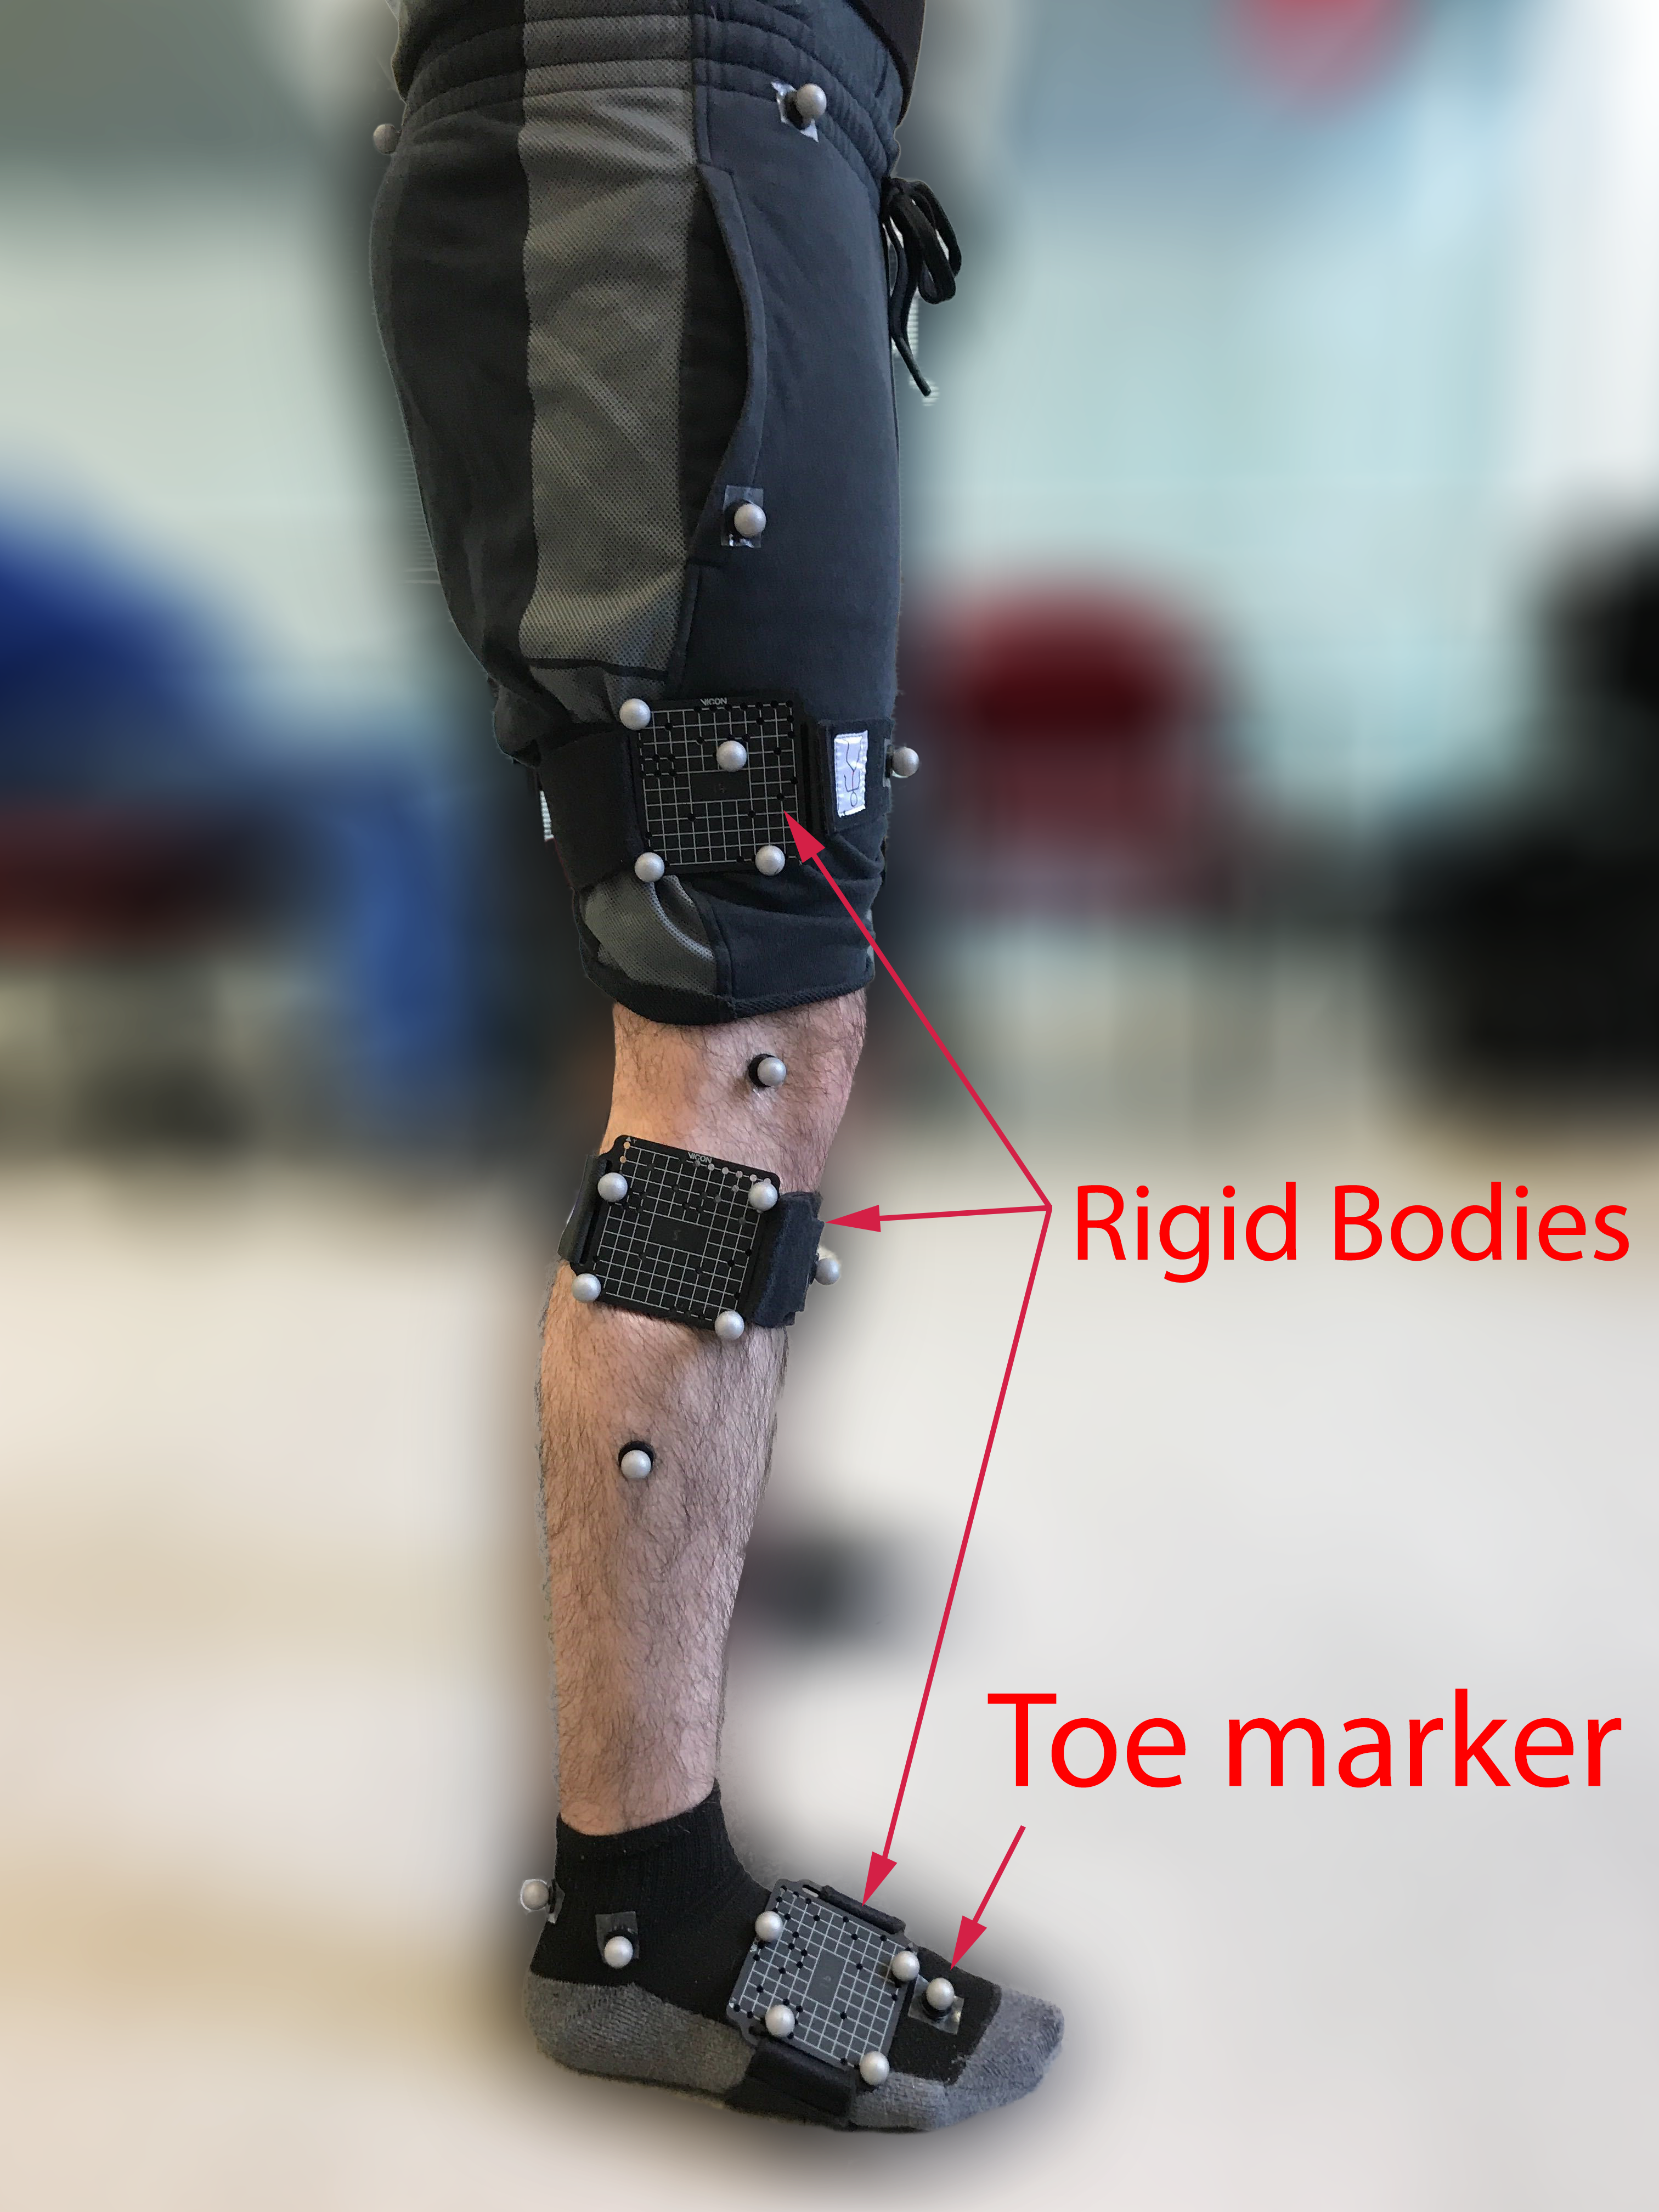
\includegraphics[scale=0.04,frame]{images/marker_side_cap.png} 
  \caption{Side view of the markers} 
  \label{fig:markers_side} 
\end{subfigure} 

\begin{subfigure}{0.5\linewidth} 
  \centering 
  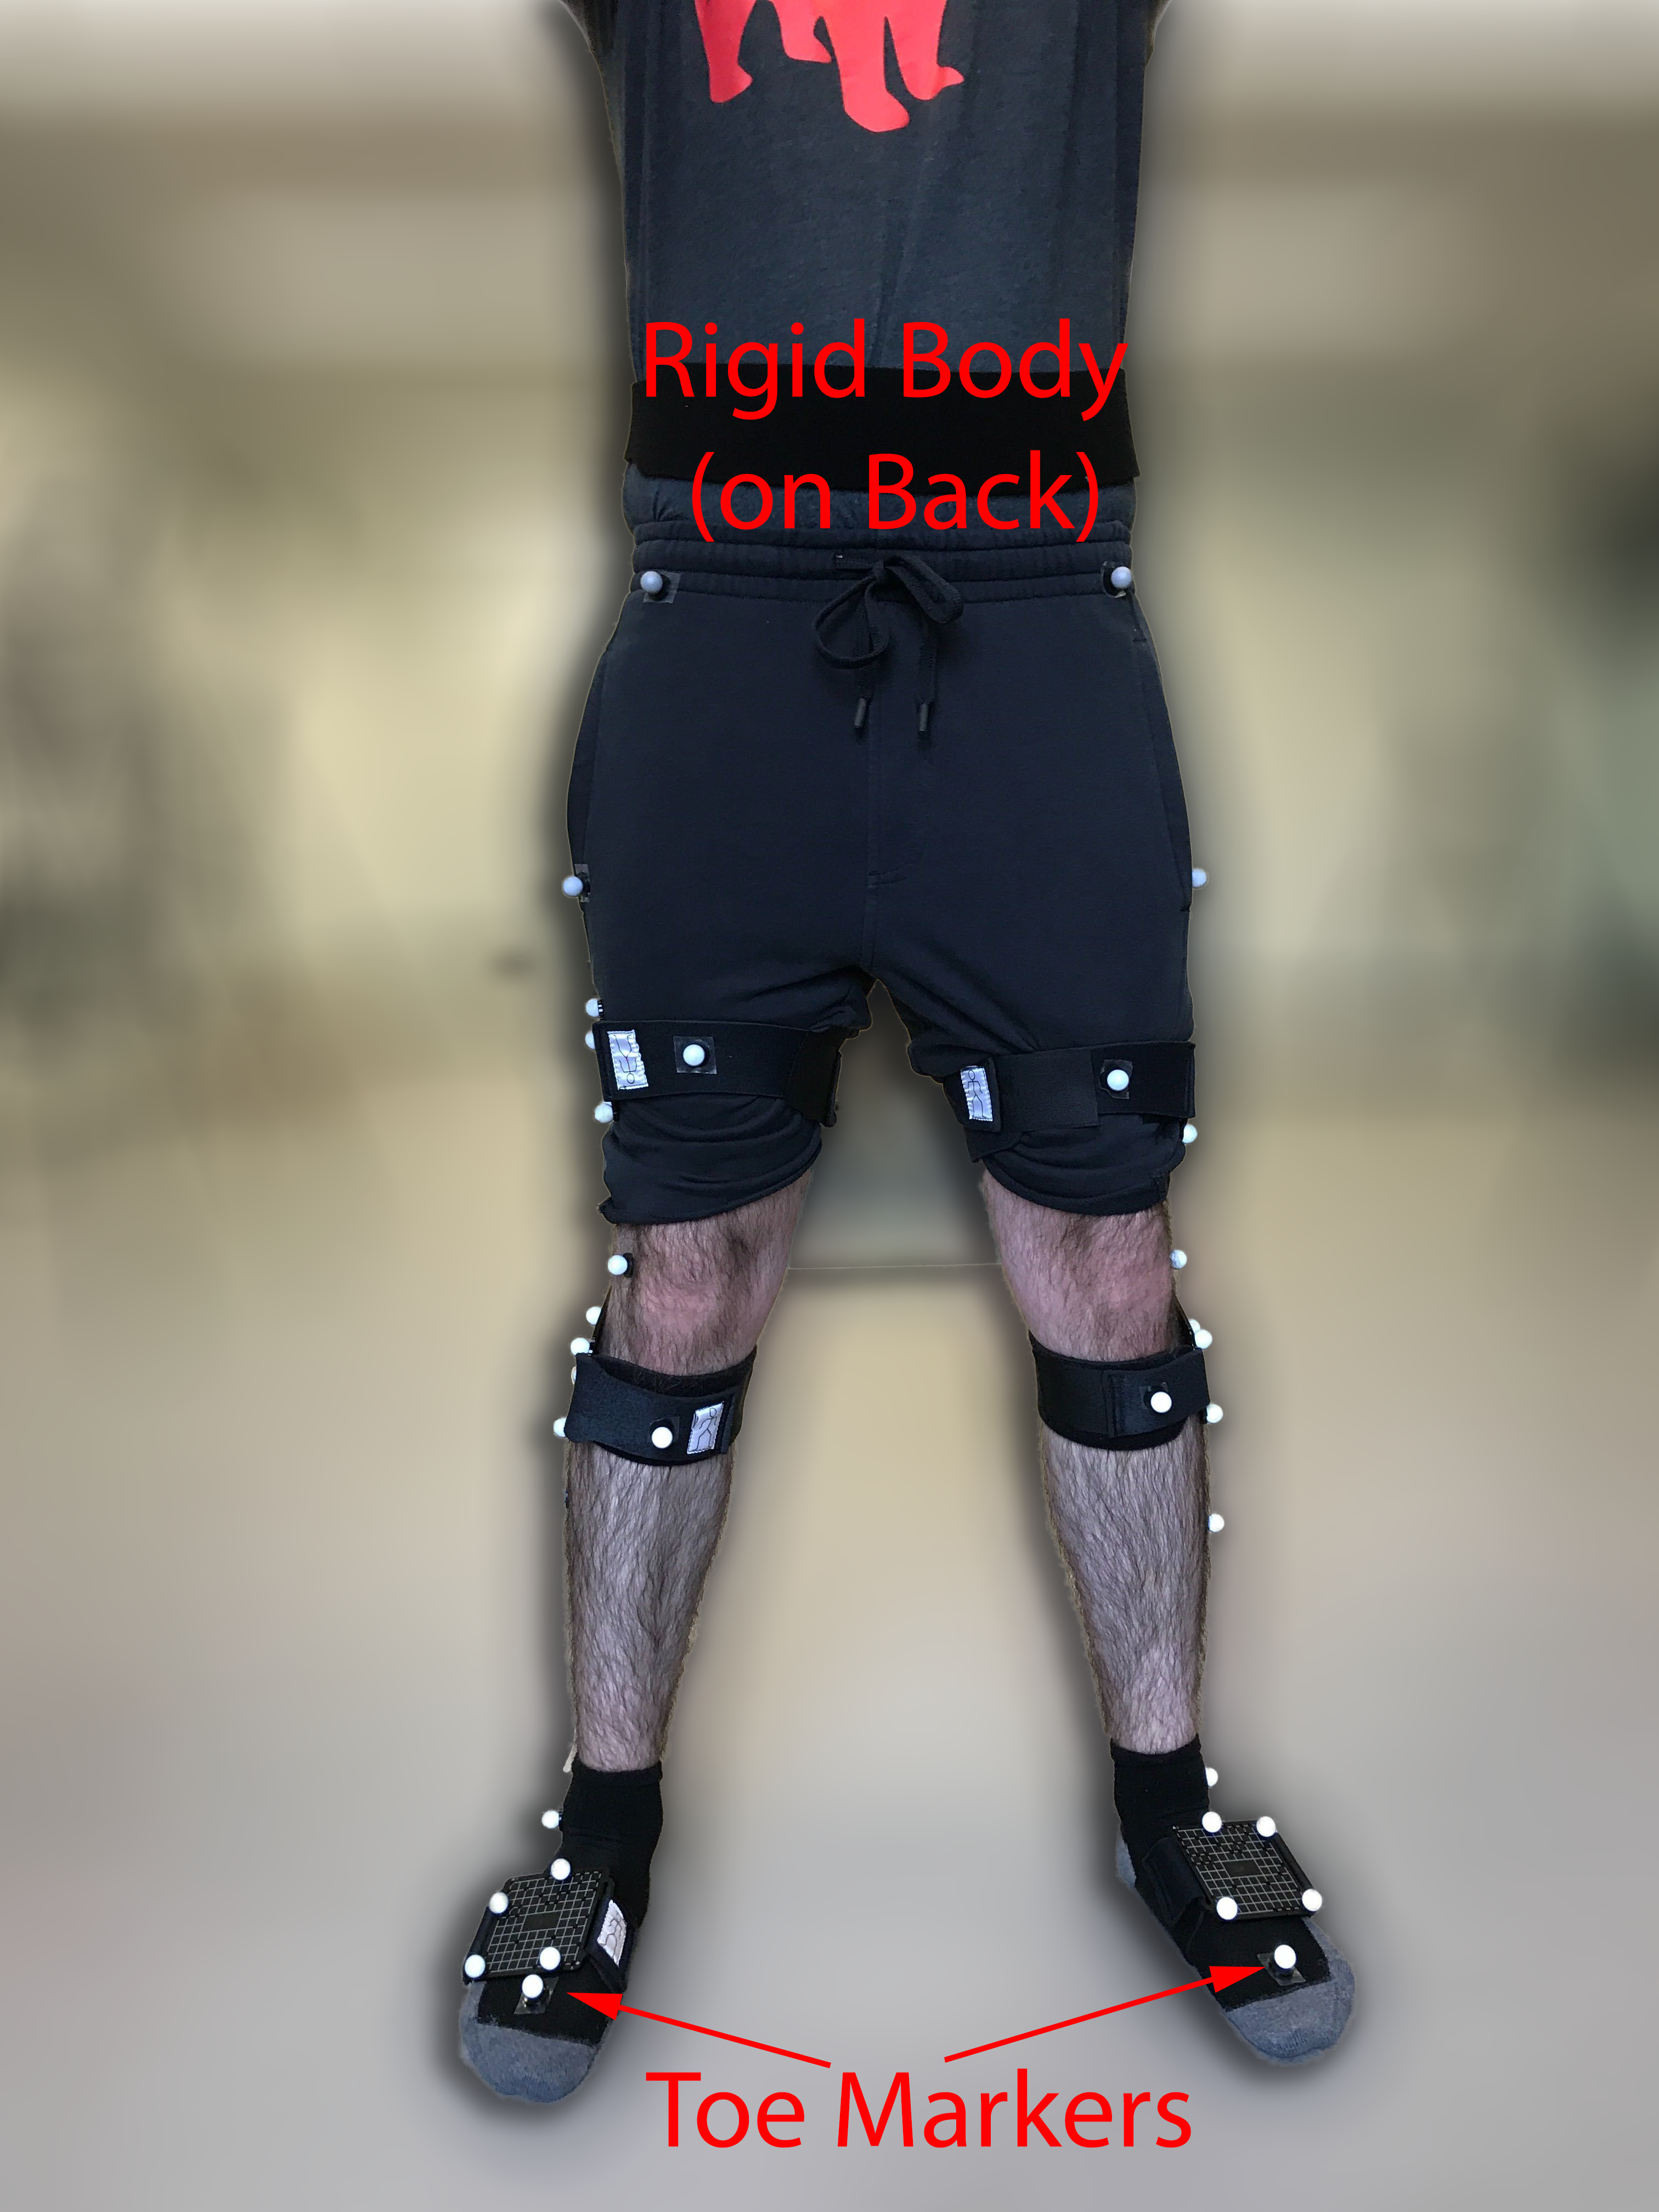
\includegraphics[scale=0.04,frame ]{images/front_markers_cap.png} 
  \caption{Front view of the markers} 
  \label{fig:markers_front} 
\end{subfigure} 
\caption{The markers were placed according to the plugin marker template. Additional rigid body plates were placed on the subjects' thighs, shanks, feet, and back.} 
\label{fig:markers} 
\vspace*{-3mm}
\end{figure} 


\begin{figure}
    \centering 
    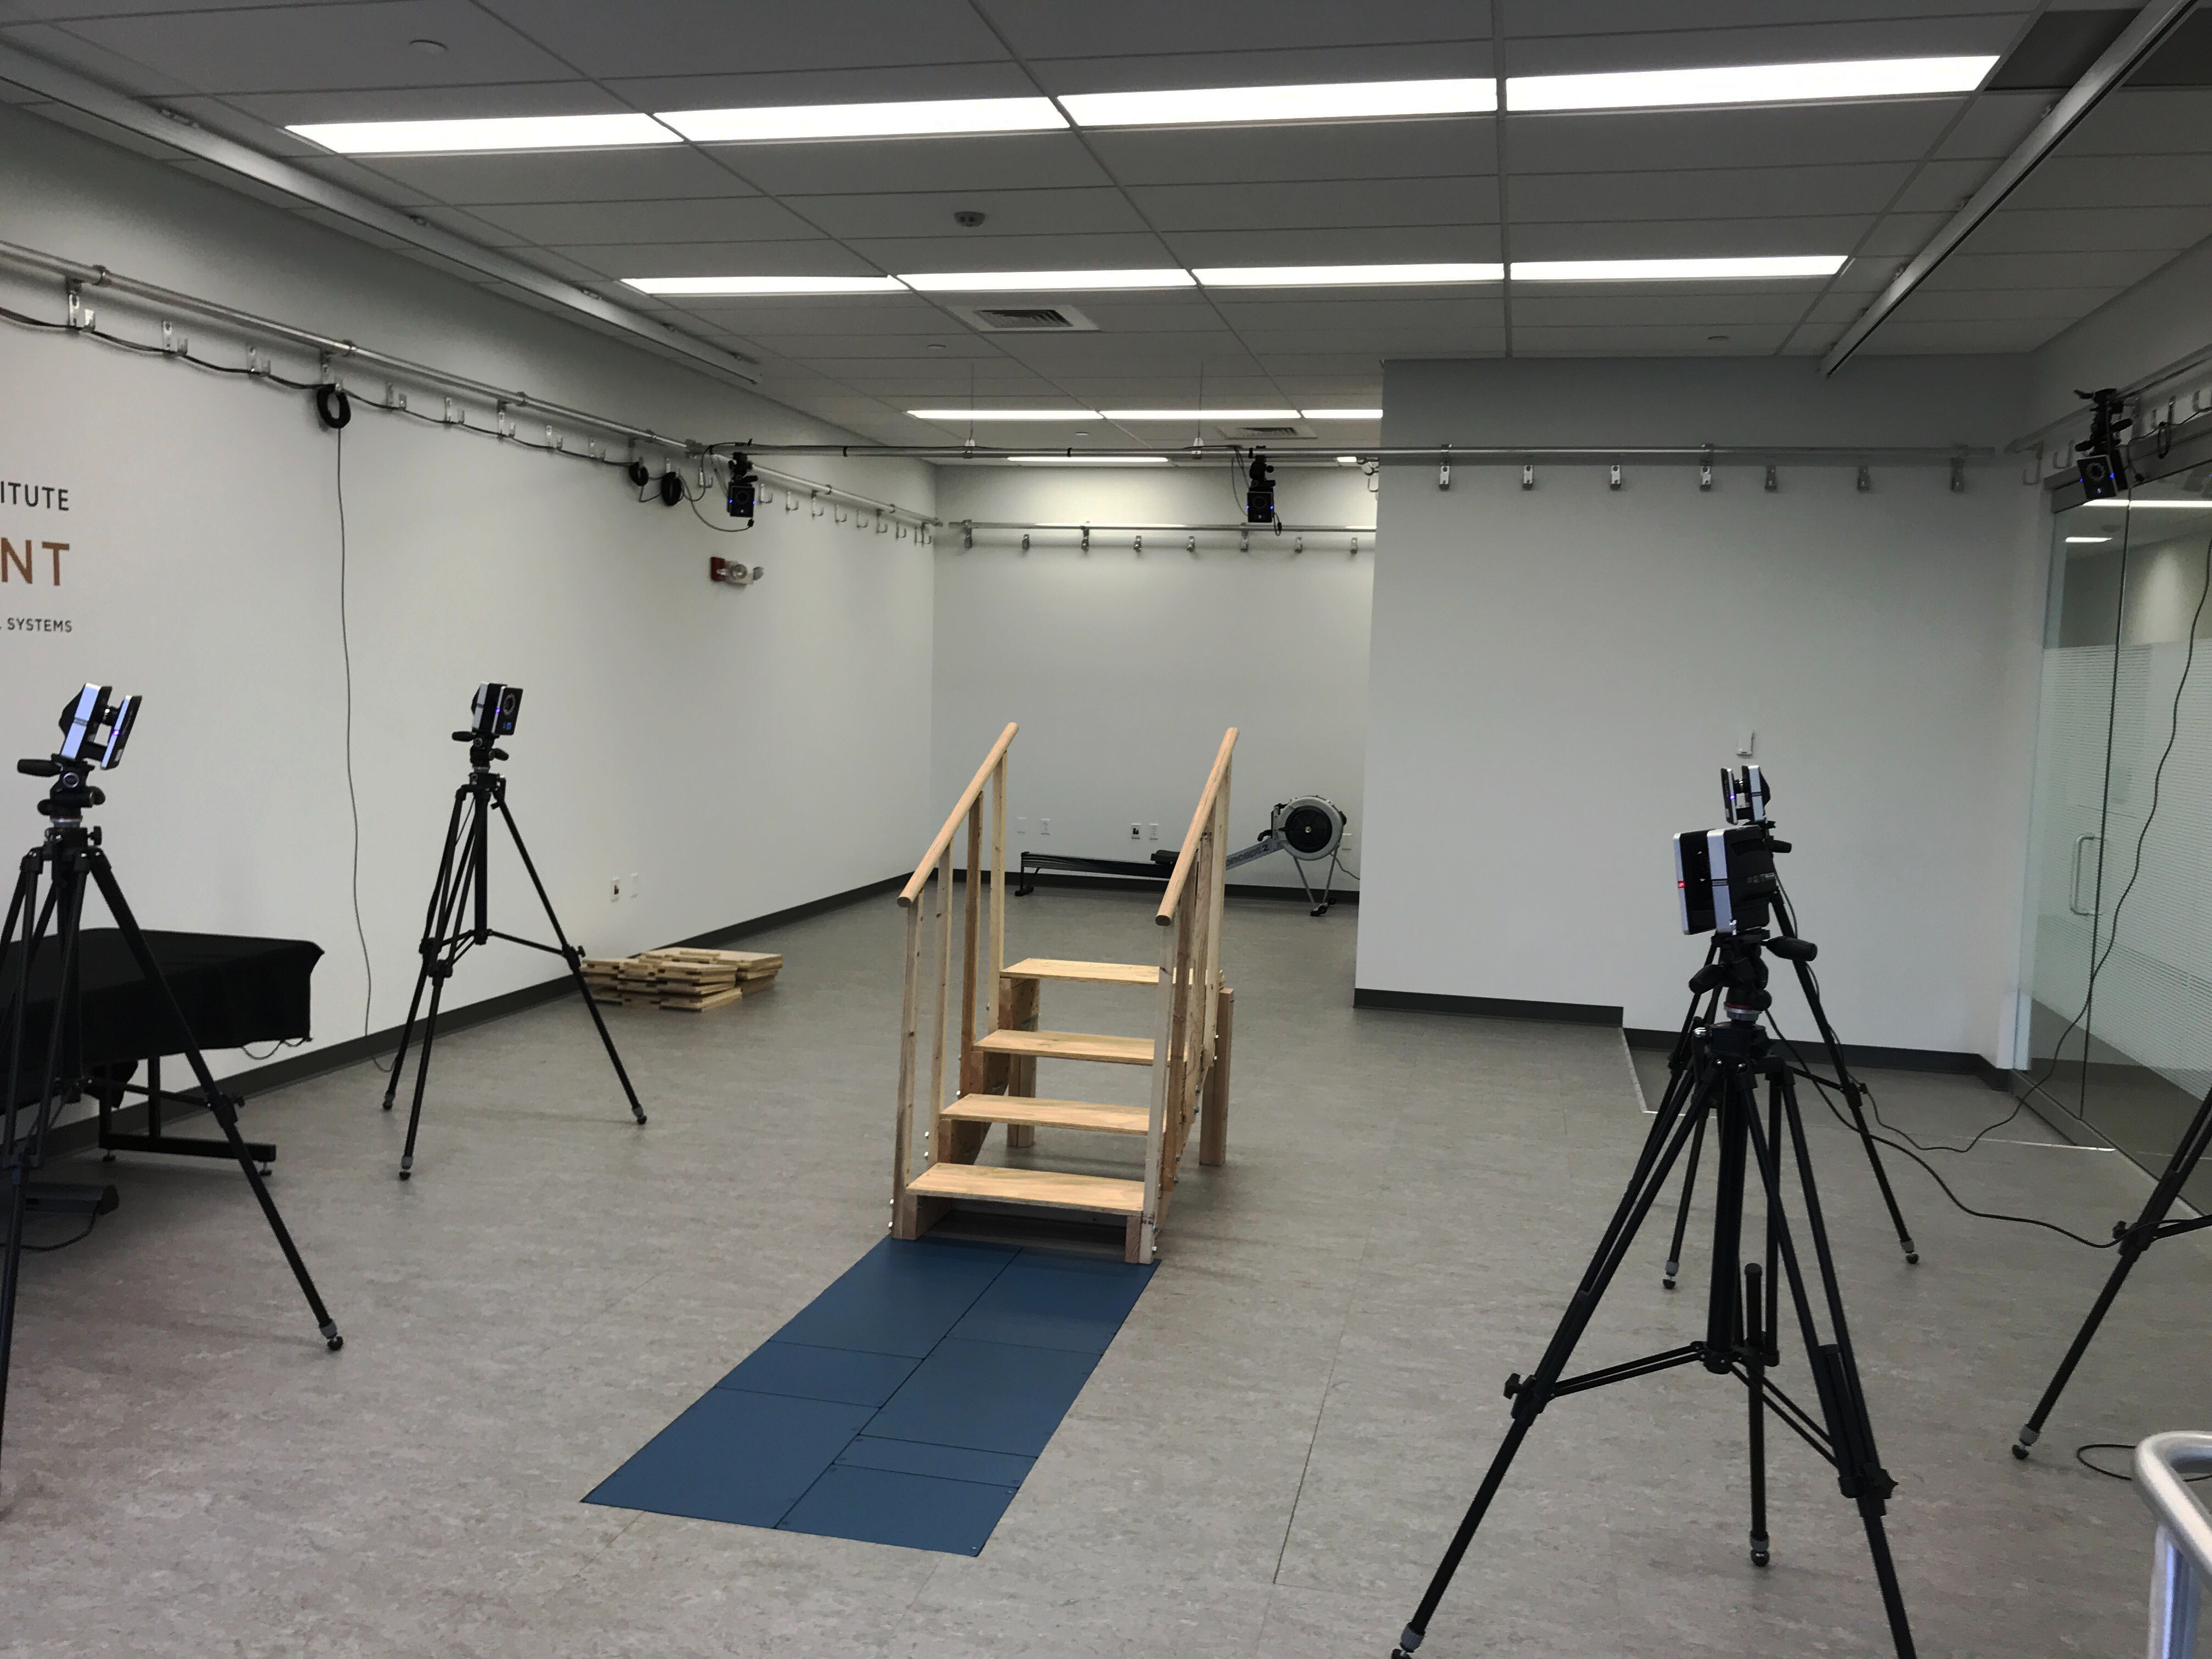
\includegraphics[scale=0.04,frame]{images/stairs.png}
    \caption{Motion capture area with custom staircases. The stairs had sliding planes to adjust the heights. Four of the mocap cameras were placed around the stairs to mitigate. marker occlusions}
    \label{fig:mocap} 
\end{figure} 

\subsection{Learning the Trajectories} 
\autoref{fig:stick} shows the coordinate layout used in this paper. The $X$ axis is perpendicular to the plane and is not considered. Exoskeletons are typically controlled in the sagittal plane, so out-of-plane motion is not required. \autoref{fig:stick} shows a diagram of the subject in motion. In this diagram, the toe's position is being controlled from the ground to the first step of the staircase. The limb lengths of the subject used for training were measured using a calibration phase. However, the limb length segments can be estimated using the height of the subject \cite{anthropomorphic}. It is assumed that the relative location of the stairs is known with respect to the person. The motion has to be transferred to joint space using inverse kinematics of the leg. To avoid a collision of the toe with the lip of the stairs, a constraint that the foot has to be parallel to the ground is imposed. In addition, some rehabilitation exoskeletons do not have actuated ankle joints and therefore cannot be controlled.  \autoref{eq:IK} is the inverse kinematics of the leg with a constrained ankle where hip: $q_1$, knee: $q_2$, ankle: $q_3$, thigh: $l_1$, shank: $l_2$, ankle height: $l_3$, foot length: $l_4$, and $z_{toe}$ and $y_{toe}$ is the coordinate of the toe. As opposed to forward kinematics, inverse kinematics allows for the encoding of the stair height. 

\begin{equation} 
    \begin{aligned} 
        y' &= y_{toe} - l_4 \\ 
        z' &= z_{toe} + l_3 \\  
        \gamma &= y'^2 - z'^2 - l_1^2  - l_2^2 \\ 
        q_2 &= atan2 \Bigg( -\sqrt{1 - \frac{\gamma }{2 l_1^2 l_2^2}}, \frac{\gamma}{2 l_1^2 l_2^2}\Bigg)\\ 
        q_1 &= (atan2(z, y) - atan2( l_2 s_{q_2}, l_1 + l_2 c_{q_2})) + 0.5\pi \\ 
        q_3 &= (2\pi - q_1 - q_2) 
    \end{aligned} 
    \label{eq:IK} 
\end{equation} 

 
\begin{figure} 
    \centering 
    \includegraphics[scale=0.75]{images/stick.png} 
    \caption{Stair climbing motion of a 3 DoF leg. The start and goal are the parameters of the model shown as the distance $d$ and height $h$ from the toe to the stair. Each of the joint angles are calculated using inverse kinematics.} 
    \label{fig:stick} 
    \vspace*{-4mm}
\end{figure} 



Dynamic Time Warping temporally aligns two demonstrations. DTW attempts to minimize the distance between two trajectories by drawing lines between the two curves \cite{muller2007dynamic} \cite{JSSv031i07}. \autoref{eq:DTW} shows the equation for DTW; it maps demo 2 onto demo 1. Here, $\delta (P, T)$ is defined as the Manhattan distance function. $P$ and $T$ are demo 2 and demo 1, respectively. This method maps $P$ onto $T$. The Euclidean distance and Manhattan distance were both examined as criteria. Here, $w_k$ is the cost at index $(i,j)$, and $k$ is the time frame. DTW does not produce smooth trajectories; the trajectories have to be smoothed so that the derivative of the trajectory can be found. A high order polynomial fit to the temporally scaled demonstrations removes the disturbance from the demonstrations.



\begin{equation} 
    \begin{aligned} 
         \delta (P,T) &= | p_i - t_j| & \text{Distance function} \\ 
        DTW(P,T) &= min \Bigg[ \sum_{k=1}^{K} \delta (w_k) \Bigg] & \text{Minimum path} 
    \end{aligned} 
    \label{eq:DTW} 
\end{equation} 


DMPs work by encoding the force profile during the trajectory. The first and second derivative of the marker trajectory is calculated to transfer the marker trajectory from position space to a forced space using a PD controller seen in \autoref{eq:force}. The gain matrices are $K_p$ and $K_d$, $g$ is the goal of the system, and $x$ is the system state. This conversion is done because the DMP controller needs a force input to drive the system.

\begin{equation}
    F = \ddot{x} - K_p (g - x) - K_d\dot{x}
    \label{eq:force}
\end{equation}



The Expectation-Maximization (EM) algorithm iteratively updates the probabilities of the points. The EM algorithm is used to find the optimal mean and covariance of each of the Gaussian. The goal of the EM algorithm is to find similar points in the demonstrations and group them together into clusters. \autoref{eq:Estep} and \autoref{eq:Mstep} show the two steps in the EM algorithm. In these equations, $X$ is the point vector, $h$ is the posture probability, $\pi$ is the weighting coefficient for each point, $\mu$ is mean, and $ \Sigma $ is the co-variance.  K-means is used to find the initial guess of the $\mu$ and $\Sigma$ parameters for the EM algorithm with the value of $\pi$ initialized randomly. The GMM/GMR code used in this paper were based on Calinon open-source libraries \cite{Calinon19MM} \cite{CalinonLee19} \cite{Calinon16JIST}. 

E(xpectation)-step: 
\begin{equation} 
     h_{t,i} = \frac{\pi_i \prod_{j=1}^{P} \mathcal{N}(X_t^j | \mu_i^j , \Sigma_i^j )}{ \sum_k^K \pi_k \prod_{j=1}^{P} \mathcal{N}(X_t^j | \mu_k^j , \Sigma_k^j ) } 
     \label{eq:Estep} 
\end{equation}{} 

M(aximization)-step: 
\begin{equation} 
\begin{aligned} 
    \pi_i &\leftarrow \frac{\sum_t^N h_{t,i}}{N} \\ 
    \mu_i^j &\leftarrow \frac{\sum_t^N h_{t,i} X_t^j}{\sum_t^N h_{t,i}} \\ 
    \Sigma_i^j &\leftarrow \frac{\sum_t^N h_{t,i} ( X_t^j - \mu_i^j)  ( X_t^j - \mu_i^j)^T   }{\sum_t^N h_{t,i}}  
\end{aligned} 
\label{eq:Mstep} 
\end{equation} 


The number of bins $ K $ can be found using the Bayesian Information Criterion (BIC). If too few bins are used, the model will be poorly fit; if too many are used, it will over-fit to the demonstrations. BIC is a method to overcome this limitation and find the optimal number of bins. \autoref{eq:BIC} calculates the BIC score; it is a trade-off between optimizing the likelihood and minimizing the number of states to encode.  $\mathcal{L}$ is the log-likelihood, $ N $ is the number of mixture models, $ K $ is the number of components, and $ D $ is the dimension of the data points. \cite{calinon2007learning, billard2006discriminative}. 


\begin{equation} 
    S_{BIC} = -\mathcal{L} + \frac{log(N)(K(D+1)(D+2)-2)}{4}  
    \label{eq:BIC} 
\end{equation} 





GMR models the regression function from the joint probabilities in the form of GMM. The GMM algorithm is a probabilistic form of the K-means algorithm. In this formulation, GMM was used to find the mean and covariance of the basis functions over the data set. GMR was used to regress over the basis function, creating the forcing function needed for the DMP. \autoref{eq:GMR_Prop} calculates the likelihood and \autoref{eq:GMR_mu} calculates the covariance and mean. $\xi_$ is a multidimensional array, $\mu_i^o$ and $\Sigma_t^o$ are vectors of the output mean and covariance, and $\mu_i^I$ and $\Sigma_t^I$ are vectors of the input mean and covariance.   \autoref{fig:GMM} shows the position of the Gaussian and force profile. There are several Gaussian on the upper graph; some are easily visible. The others have small eigenvalues, creating an eclipse with small areas. The blue lines are the training force profiles, with the red line being the learned force profile.   

\begin{equation} 
     P(\xi_t^O | \xi_t^I ) \sim \sum_i^K h_i(\xi_t^I) \mathcal{N}( \hat{\mu_i^o}, \hat{\Sigma_t^o}) 
     \label{eq:GMR_Prop} 
\end{equation} 

where, 

\begin{equation} 
    \begin{aligned} 
      \hat{\mu_i^o} &= \mu_i^o + \Sigma_i^{OI}\Sigma_i^{I-1}(\xi_t^I - \mu_i^I)\\ 
      \hat{\Sigma_i^O} &= \Sigma_i^O - \Sigma_i^{OI}\Sigma_i^{I-1}(\xi_t^I - \mu_i^I) \\ 
       h_{i} &= \frac{\pi_i \mathcal{N}(\xi_t^I | \mu_i^j , \Sigma_i^j )}{ \sum_k^K \pi_k \mathcal{N}(\xi_t^I | \mu_k^j , \Sigma_k^j ) }   
    \end{aligned} 
    \label{eq:GMR_mu} 
\end{equation} 

DMPs allow for the manipulation of the encoded trajectories. \autoref{eq:DMP} shows the basic formulation of the DMPs. The force function $f$ is calculated from GMR and drives the function, $\beta_y$ and $\alpha_y$ are the system gains, $y$ is the system state, and $g$ is the goal. \autoref{eq:canonical} shows the canonical system. $\tau$ is a time constant and $\alpha_x$ is a constant term. It models the generic behavior of the model. The $\tau$ term is used for scaling the trajectories in time.  


\begin{equation}
    \tau \ddot{y} = \alpha_x (\beta_y(g-x)-\dot{y}) + f  
    \label{eq:DMP} 
\end{equation}


\begin{equation}
    \tau \dot{x} = -\alpha_x x  
    \label{eq:canonical} 
\end{equation}



A reproduction model's accuracy can be measured by calculating the imitation cost. This is essentially a root mean squared algorithm that measures how well the model follows the demonstrations \cite{metric}. \autoref{eq:metric} shows the equation used to calculate the goodness of fit. In this equation, $d$ is the demo, $m$ is each of the demos, $t$ is the time, and $x$ is the trained model. All of the demonstrations were first aligned using DTW.

   \begin{equation}
        C = \frac{1}{MT} \sum_m^M{\sum_t^T{ || d^m_t - x_t||}}
        \label{eq:metric}
    \end{equation}



\section{Results}

Data was collected on the trajectories of the eleven subjects from the lowest stair configuration (config0). Eight subjects were randomly selected to train the model. The remaining three subjects were used for validation. No additional prepossessing of the mocap data was required except for the gap-filling done in the Vicon Nexus software. 

\autoref{fig:ytraj} and \autoref{fig:ztraj} compare the $Y$ and $Z$ positions of the right leg's toe marker for the eight validation subjects. Each of the trajectories shown in these graphs was input as a training demonstration for the model. Each of the subjects climbed at different speeds, but follow a similar trajectory. The trajectories were aligned using Dynamic Time Warping to solve the speed inconsistency, this scaling removed the time dependencies of the trajectories. This is shown in the time-normalized variable $s$, where $s$ 0 $\rightarrow$ 1. A temporally-scaled trajectory is not continuous; the trajectories contain jagged segments and are thus not differentiable. A high order polynomial smoothed each warped trajectory to ensure that it is continually differentiable. The $Y$ trajectories have different ending positions; this can be accounted for by the subject's different gaits. This variation allows the model to adapt. In addition, using DMPs allows for the abstraction of the goal. The trajectories can be scaled in time using the $\tau$ parameter. When $\tau$ is 1, the trajectory is reproduced in real time. To speed up the system, increase $\tau$ above 1. To slow it down, decrease it to less than 1.  

\begin{figure}[h]

    \begin{subfigure}{\linewidth}
        \centering 
        \includegraphics[ scale=0.5]{images/ytraj_s.png} 
        \caption{The toe marker $Y$ position trajectories} 
        \label{fig:ytraj} 
    \end{subfigure} 

    \begin{subfigure}{\linewidth}
        \centering 
        \includegraphics[ scale=0.5]{images/ztraj_s.png} 
        \caption{The toe marker $Z$ position trajectories} 
        \label{fig:ztraj} 
    \end{subfigure} 
    \caption{Comparison of different subjects' climbing motion in the sagittal plane. Each line is the motion from a different subject's trial.}
    \label{fig:trainingDemos}
\end{figure}

\autoref{fig:DTW} shows the alignment of a trajectory against a demonstration. The blue line is demo 1, and the orange line is demo 2. DTW aligns demo 2 with demo 1. The green line represents the aligned trajectory and the red line represents a polynomial fit to the aligned trajectory. The cost map shows the closest fit of points from $P$ to $T$. The white spots are the hills and the black spots are the valleys, with the path being the minimum cost from start to goal. The total path cost associated with the Euclidean was $17652.35$, and the cost of the Manhattan path was $33.50$. This is the cost of aligning the demonstration with the model trajectory. The Manhattan metric had a much lower cost than the Euclidean metric, allowing for a better fit. 



% \begin{figure} [h]
%     \centering 
%     \includegraphics[frame, scale=0.5]{images/ytraj.png} 
%     \caption{Subject Y Trajectories} 
%     \label{fig:ytraj} 
% \end{figure} 

% \begin{figure} [h]
%     \centering 
%     \includegraphics[frame, scale=0.5]{images/ztraj.png} 
%     \caption{Subject Z Trajectories} 
%     \label{fig:ztraj} 
% \end{figure} 


\begin{figure}[h]
     \centering 
     \includegraphics[ scale=0.12]{images/DTW_annotated.png} 
     \caption{Two demos being aligned using DTW and a smoothed trajectory. Blue line: demo 1. Orange line: demo 2. Green line: aligned trajectory. Red line: Polynomial smooth trajectory. The cost map shows the distance between the points.} 
     \label{fig:DTW} 
       \vspace*{-4mm}
\end{figure} 
 
\autoref{fig:BIC} shows the BIC score calculated for several bin sizes (1-24) for the $ Y $ and $ Z $ trajectories of the toe marker. This calculation limits the number of bins. The two graphs are generated using a single demonstration from each of the eight subjects in the config0 data set. The optimal number of bins for the $Z$ axis is 6 bins and the optimal number of bins for the $Y$ axis is 7 bins.


\begin{figure}[h]
   \begin{subfigure}{\linewidth} 
    \centering 
    \includegraphics[ scale=0.48]{images/ybic7.png} 
    \caption{BIC score for toe marker $Y$ position trajectory. The BIC score has its first local minimum at a size of 7 bins.} 
    \label{fig:BICY} 
  \end{subfigure}  

   
\begin{subfigure}{\linewidth} 
    \centering 
    \includegraphics[ scale=0.48]{images/zbic6.png} 
    \caption{BIC score for toe marker $Z$ position trajectory. The BIC score has its first local minimum at a size of 6 bins.} 
    \label{fig:BICZ} 
  \end{subfigure}  
    \caption{The BIC score (smaller is better) was calculated for numerous bins size for the $Y$ and $Z$ trajectory.} 
    \label{fig:BIC} 
      \vspace*{-5mm}

\end{figure}  


\autoref{fig:GMM} shows the placement of the Gaussian on the learned forcing function for the $Z$ axis. Only one axis is reported to illustrate how the underlining model is created. The blue lines are the demonstrations of forcing functions and the yellow line is the learned forcing function. The green ovals are the Gaussian, and the red dots are the means of the Gaussian. This graph shows the areas of correlation among the demonstrations. The location of the Gaussian was determined by the EM step in the GMM algorithm, and the yellow line is the forcing function calculated by the GMR algorithm that regresses the Gaussian.    



\begin{figure}[h]
    \centering 
    \includegraphics[ scale=0.13]{images/forcing_func_large.png} 
    \caption{The Gaussian positions over the demonstrations and the learned forcing function for the $Z$ axis. The blue lines are the demonstrations, the yellow line represents the learned mode, and the Gaussian is in the green ovals with the red dot as the mean of the Gaussian. The figure shows a zoomed-in Gaussian for comparison.} 
    \label{fig:GMM} 
\end{figure} 


\autoref{fig:trajLearning} shows the result of the learning of the $Y$ and $Z$ models using config0 subject data. The thick lines represent the generated model that was learned from the demonstrations using the optimal number of bins and demonstrations. The oscillations are caused by the DTW fitting of the demonstrations and the polynomial smoothing. The demonstrations with few points are being fit to the models with more points. The polynomial fitting ensures that the trajectories are smooth and not jagged.


\begin{figure}[h] 
  \centering 
  \begin{subfigure}{\linewidth} 
    \centering 
    \includegraphics[ scale=0.50]{images/ylearn7.png} 
    \caption{Comparison of learning the $Y$ marker position trajectory} 
    \label{fig:compY} 
  \end{subfigure} 
  \begin{subfigure}{\linewidth} 
    \centering 
    \includegraphics[ scale=0.50]{images/zlearn6.png} 
    \caption{Comparison of learning the $Z$ marker position trajectory} 
    \label{fig:compZ} 
  \end{subfigure}   
  \caption{Imitation model for the toe position for climbing a stair. The $Z$ position is height of the toe relative to the floor and the $Y$ position is where the toe lands relative to the body. The thick line is the imitation model. The models used the optimized number of bins calculated from the BIC score.} 
  \label{fig:trajLearning} 
    \vspace*{-2mm}
\end{figure}   


\autoref{fig:compare_methods} shows an example trajectory compared to that of a model trained from the motion of only a single subject and the model trained on all eight subjects. \autoref{tab:error} shows the imitation cost for a model trained with a single subject and a model trained using multiple subjects (see \autoref{eq:metric}). Both models were compared against a demonstration that was not used to train either model.  


% \begin{figure} 
%     \centering 
%     \includegraphics[frame, scale=0.5]{images/compy.png} 
%     \caption{Multiple vs single examples for Toe(Y) trajectory} 
%     \label{fig:compare_methodsy} 
% \end{figure} 

% \begin{figure} 
%     \centering 
%     \includegraphics[frame, scale=0.5]{images/compz.png} 
%     \caption{Multiple vs single examples for Toe(Z) trajectory} 
%     \label{fig:compare_methodsz} 
% \end{figure} 

% \begin{figure}[h]
%     \centering
%     \begin{subfigure} {\linewidth} 
%         \centering 
%         \includegraphics[frame, scale=0.5]{images/compy.png} 
%         \caption{Multiple vs single examples for Toe(Y) trajectory} 
%         \label{fig:compare_methodsy} 
%     \end{subfigure} 
% 
%     \begin{subfigure} {\linewidth} 
%         \centering 
%         \includegraphics[frame, scale=0.5]{images/compz.png} 
%         \caption{Multiple vs single examples for Toe(Z) trajectory} 
%         \label{fig:compare_methodsz} 
%     \end{subfigure} 
%     \caption{Comparison of a demonstration against a model trained on a single demonstration and a model trained on multiple demonstrations.}
%     \label{fig:comparison}
% \end{figure}

\begin{figure}[h]
    \centering 
    \includegraphics[scale=0.20]{images/compare_method.png} 
    \caption{Comparison of a demonstration against a model trained on a single demonstration and a model trained on multiple demonstrations. This is expressed over frames. } 
    \label{fig:compare_methods} 
\end{figure} 

\begin{table}[h]
\large 
     \centering 
     \begin{tabular}{||c|| c c ||}  
     \hline 
         Axis     & Y & Z  \\ [0.5ex]  
         \hline\hline 
         Single subject   & 138.01 & 67.86  \\  
         \hline 
         Multiple subjects & 70.7 & 25.63  \\ 
         \hline      
     \end{tabular} 
     \caption{Imitation cost (smaller is better) comparing models trained on a single subject to that trained on multiple subjects. The compared trajectories are shown in \autoref{fig:compare_methods}. } 
     \label{tab:error} 
\end{table} 


\autoref{fig:singleSubject} shows the training and reproduction of the models trained on different stair heights. The solid line is the raw trajectory, and the dotted line is the reproduced line. To test the model's ability to adapt to different stair heights, the goal($g$) of the model was changed to each of the different stair heights. For example, for the model trained on a trajectory whose end position (goal) was $250mm$, the goal was changed to a height of $275mm$. The model is able to follow a foot trajectory for a different stair height. This trajectory was not one of the demonstrations used to train the model.


\begin{figure}
    \centering
    \includegraphics[scale=0.20]{images/compareHeihgts.png}
    \caption{A model trained on a single subject and single configuration, reproducing the motion climbing different stair heights. The solid lines are the marker trajectories. The dotted lines are the reproduced trajectories using the model.}
    \label{fig:singleSubject}
\end{figure}

% \begin{figure}[h]
%   \centering 
%   \begin{subfigure}{\linewidth} 
%     \centering 
%     \includegraphics[frame, scale=0.17]{images/config0.png} 
%     \caption{Using config0 to learn} 
%     \label{fig:config0} 
%   \end{subfigure} 
%     \begin{subfigure}{\linewidth} 
%     \centering 
%     \includegraphics[frame, scale=0.17]{images/config3.png} 
%     \caption{Using config3 to learn} 
%     \label{fig:config3} 
%   \end{subfigure}   
%   \caption{A model trained on single subject and single configuration, reproducing the motion climbing different stair heights. The solid lines are the marker trajectories. The dotted lines are the reproduced trajectories using the model \autoref{fig:config3} that was trained on stair config3. The dotted lines should converge to the solid lines.} 
%   \label{fig:singleSubject} 
% \end{figure}   


Using the inverse kinematics and the anthropomorphic parameters, the joint angle can be calculated. \autoref{fig:stairsclimbing} shows the movement of the leg through a stepping trajectory. The trajectory of the toe is being controlled. The joint angles at each instance are determined using inverse kinematics. The ankle is constrained to be parallel to the ground. This constraint is to prevent the toe from catching on the edge of the stairs.


% \begin{figure}
%     \centering
%     \includegraphics[scale=0.20]{images/stairs_climb.png}
%     \caption{The leg motion over the stepping trajectory while keeping the ankle parallel with the ground. Inverse kinematics was then used to solve for the joint angles.}
%     \label{fig:stairsclimbing}
% \end{figure}

\begin{figure}[h!]
  \centering 
  \begin{subfigure}{\linewidth} 
    \centering
    \includegraphics[scale=0.20]{images/stairs_climb.png}
    \caption{The leg motion over the stepping trajectory while keeping the ankle parallel with the ground. Inverse kinematics was then used to solve for the joint angles.}
    \label{fig:stairsclimbing}
  \end{subfigure} 
    \begin{subfigure}{\linewidth} 
    \centering 
    \includegraphics[ scale=0.20]{images/joint_angle_stairs_no_ankle.png} 
    \caption{Comparison of the joint angle. The IK path was calculated using the inverse kinematics and the toe tip. The measured joint angles are independently measured using the Vicon tracking software.}  
    \label{fig:config3} 
  \end{subfigure}   
  \caption{Control of the leg from the ground to the first step. The joint angle are calculated and compared to the measured joint angles. } 
  \label{fig:singleSubject} 
\end{figure}   

% \begin{figure}
%     \centering 
%     \includegraphics[frame, scale=0.16]{images/climbing_stair.png} 
%     \caption{The leg motion over the stepping trajectory while keeping the ankle parallel with the ground. Inverse kinematics was then used to solve for the joint angles.} 
%     \label{fig:stairsclimbing} 
% \end{figure} 


\section{Discussion} 
The trajectory of the foot for each subject follows a similar trajectory in the plane as referenced in \autoref{fig:stick}. The $Y$ position varied among the subjects and stair configurations. The subjects had different heights, which affects their stride length. This variation along the path is encoded during the GMM processes. The DMP formulation abstracts the start and goal of the trajectories. The locations of the start and goal positions have to be determined using the dynamics of the system. The $Z$ position varies very little between the subject. This is expected since each subject started on the ground and moved to the same height of the stair. The imitation model was able to replicate the trajectories from the demonstrations. 

The smoothing of the DTW trajectory is essential, as shown in \autoref{fig:DTW}. The warped trajectory contains jagged sections, which results in poor fitting and placement of the Gaussian. The demonstrations used to train the forcing function should be smooth to ensure a smooth forcing model. A polynomial was used to smooth the trajectory. 

% Specifically, there was a difference of $264mm$ between the subjects. However, the shape of the trajectories is still consistent. 

% The K-means step randomizes the initial condition; this randomization causes slight variations in the Gaussians' placement. However, it does not have a great effect on the forcing function. If too many bins are used, then extra Gaussians will be overfitted, and place Gaussian with larger covariance matrices on the demonstration data. Since the forcing function is modeled by regressing over the Gaussians, the forcing function will cause the model movements to vary from the trained path. If too little bins are used, the Gaussian will attempt to group a large number of data points into a bin. Underfitting results in the forcing function missing portions of the demonstration.     

An imitation model's accuracy can be increased by using more subject demonstrations from a single stair configuration to train a model. The cost of imitation was lower for the model trained with multiple demonstrations than a model trained with only a single demonstration. The imitation model can be lowered by increasing the number of demonstrations used to build the model. Using the BIC score, the optimal number of bins can be determined to train the model. It is important to use the optimal number of bins, or else the data will be skewed.  

This method can replicate and abstract trajectories so they can be used to climb stairs of different heights. The proximity and shape of the stairs can be found using a variety of sensors including: LIDARs, cameras, or proximity sensors. The starting and goal location must be predetermined and measured to ensure stability. The imitation model that was built was able to track trajectories from the start to the goal. Using inverse kinematics the joint angles are found to control the exoskeleton or bipedal system. The hip and knee trajectories track the measured joint angles using mocap. 


% However, the model varied from an example trajectory during reproduction. The section of the curve seems to align with the section of the Gaussian with the largest covariance. 
\section{Conclusion and Future Work} 
\label{sec:conclusion}
This paper showed how to build an imitation model by learning stair climbing trajectories using mocap and GMM/GMR. This work showed a trajectory generation of the joint motion for the exoskeleton's joint to be generalized so it can be used by people of all leg lengths on variable stair heights. Increasing the amount of subjects can improve the robustness of the model. To climb the stairs, the left and right feet take turns ascending to the same step. The trajectories were trained on subjects of different heights, ages, and genders. By training in task space, only the location of the toe is required. The joint angles are calculated using inverse kinematics and the height of the person wearing the exoskeleton. This can also be applied to a bipedal walking robot to train it to climb stairs. Future research can explore out-of-plane movement using a similar framework. 

The model can handle different stair heights by changing the start and goal inputs.  The model was optimized using the Bayesian information criterion to find the correct number of bins. This score ensured that the forcing function was not over or under fitted to the data set. The next step is to integrate a motion controller for the exoskeleton to generate the necessary torques. Integrating a sensor to detect the stair location will prevent collisions and automatically generate the start and goal positions for the trajectory generation.  

All data used in this paper is available here: \url{https://github.com/WPI-AIM/AIM_GaitData.git}
The code for extracting, analyzing, and modeling is located here: \url{https://github.com/WPI-AIM/AIM\_GaitAnalysisToolkit}




\section{Acknowledgments}
We would like to thank Chris Nycz for his time and use of the motion capture suite at the Practice Point Facility and for his constructive comments and suggestions. We would also like to thank Albert Enyedy, Lakshay Gopalka, Richard Hosea, and Nagarjun Vinukonda for running the trials. Nathaniel Goldfarb is supported by the SMART fellowship. The authors do not have any personal or financial conflicts of interest.  


\bibliographystyle{IEEEtran}
\bibliography{ref}




\end{document}
